% ------------------------- MAIN TASK ---------------------------------
\section{Reprise du projet}
\paragraph{Le projet à été repris d'un ancien collègue, dont le cahier des charges initial était :}

Concevoir un système pouvant reconnaitre des formes simples à l’aide d’une caméra, et de la librairie OpenCV, et de pouvoir implémenter cela sur un Raspberry Pi.

\subsection{État initial du projet repris}
\paragraph{La version finale du projet repris était :} Forme non-achevée du code permettant de reconnaître des formes simples. Cependant, début de travail.

\subsection{Méthode et objectifs de la reprise}
L'objectif final du projet est d'avoir un code capable de dessiner les contours des formes.
La prochaine étape de ce projet consistera à finaliser le code de reconnaissance des formes simples. Ce code sera capable de reconnaître des formes telles qu'un cercle, un carré ou un triangle, et d'afficher leurs noms soit sur une interface graphique, soit dans une console.
Une fois que ce code sera développé, veuillez vous référer au cahier des charges (voir annexe) pour le reste des tâches de ce projet.

Pour la suite du projet, j'ai décidé de choisi le langage Python, car elle permet une approche plus simple de ce genre d'algorithme et est plus facilement implémentable sur raspberry.

\paragraph{Objectifs :}
Mon objectif est dans un premier temps de faire fonctionner le code de reconnaissance d'image avec des formes simples issues d'une base de donnée, puis de l'étendre pour des images plus complexes et réelles.


%---
\clearpage
\section{Programmation Python}
A des fins de simplification, j'ai décidé d'utiliser la distribution python Anaconda, qui permet de plus simplement gérer les paquets afin de mieux traiter les différentes dépendances, concurrent direct de pip.

\subsection{Implémentation OpenCV}
La librairie de python-opencv n'est qu'une enveloppe autour du code C/C++ original. Il est normalement utilisé pour combiner les meilleures caractéristiques des deux langages, la performance de C/C++ et la simplicité de Python.

\paragraph{Installation d'open-cv :}
\begin{verbatim}
	conda install -c conda-forge opencv
\end{verbatim}
En plus de ce package, j'utiliserais d'autres tels que numpy, matplotlib etc... (Voir fichier \textit{requirements.txt} dans dossier projets).

\subsection{Reconnaissance de formes - dataset}
	Pour commencer, j'ai donc décidé de reconnaitre des formes simples, à partir d'une base de donnée avec des images de forme épurées.
	\subsubsection{Base de donnée}
	Pour ce faire, j'ai utiliser la base de donnée "2D geometric shapes dataset – for machine learning and pattern recognition"\footnote{\verb|https://www.sciencedirect.com/science/article/pii/S2352340920309847|}La base de donnée est certes grande par rapport à comment je compte l'utiliser, sachant que je n'entraine pas un model, mais elle me permettra de faire des batch de test en sélectionnant aléatoirement des images, afin de mesurer la qualité de mon algorithme selon les différents hyper-paramètres selon plusieurs formes couleurs et contrastes.
	
	\paragraph{Caractéristiques de la base de donnée :}
	
	Formes; triangle, carré, pentagone, hexagone, heptagone, octogone, nonagone, cercle et étoile
	\begin{center}
		\begin{tabular}{l|l}
			Couleur & RGB \\
			Taille & 200x200 pixels \\
			Nombre d'images & 10'000 \\
			Rotation & -180°/+180° \\
		\end{tabular}	
	\end{center}
	\clearpage
	
	\subsubsection{Explication du code}
	L'objectif de ce code est de tester mon premier algorithme de reconnaissance de formes. 
	
	\begin{figure}[!h]
		\centering
		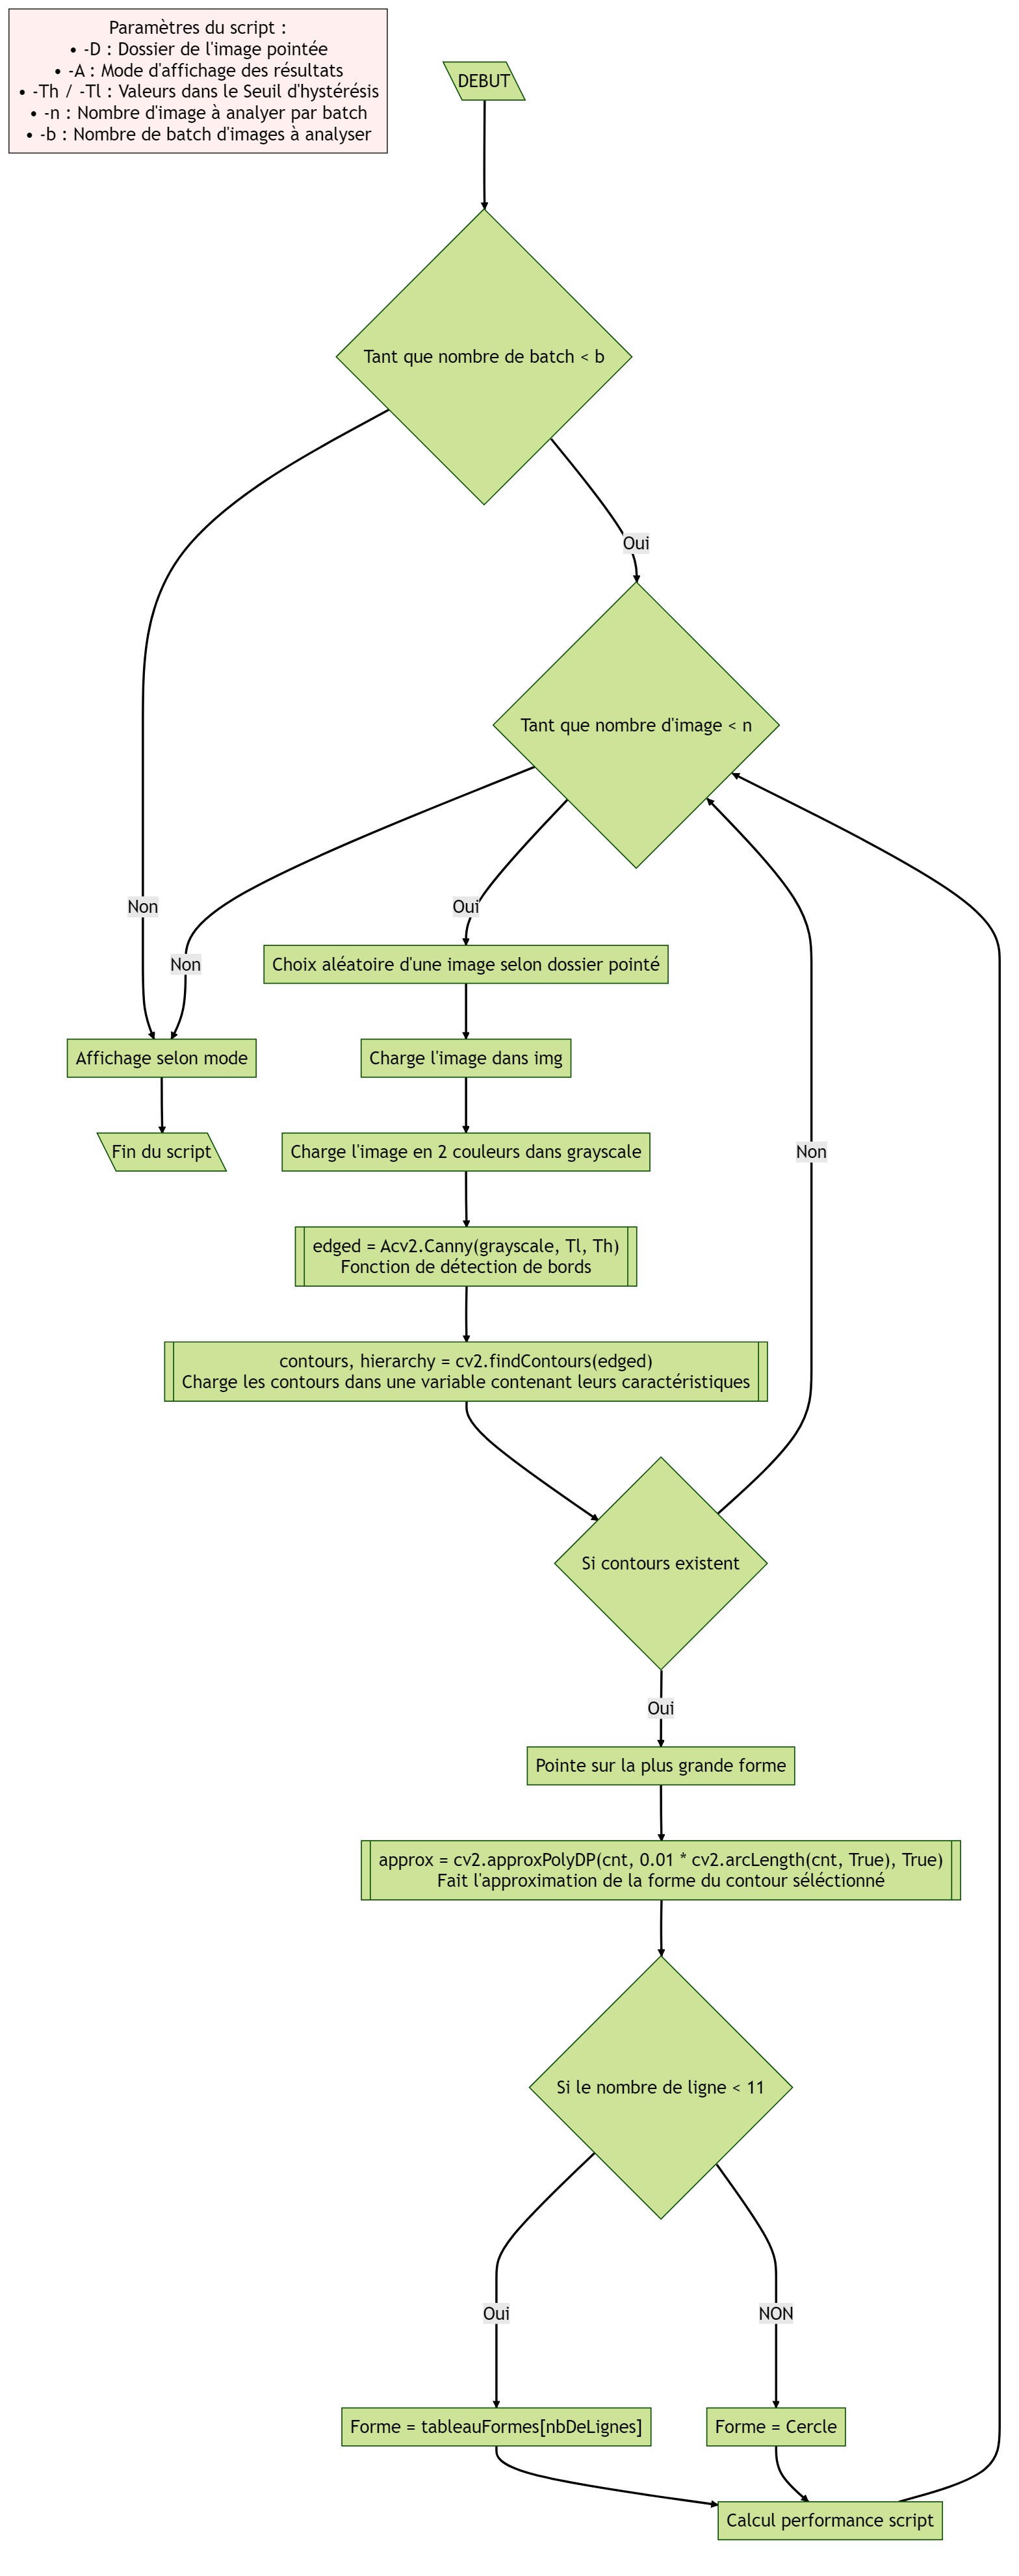
\includegraphics[height=1.2\textwidth]{../Flowcharts/ShapeDetect_B.png}
		\caption{Structogramme reconnaissance d'images}
		\label{fig:structo1}
	\end{figure}
	
	
	\subsubsection{Essais et étalonnage}
	Par la suite, j'ai pus obtenir des batteries d'analyses d'images comme sur la figure \ref{fig:batchexemple} avec des statistiques de réussites, ce qui m'a permis d'optimiser mes hyper-paramètres afin de calibrer mon algorithme.
	\begin{figure}[h]
		\centering
		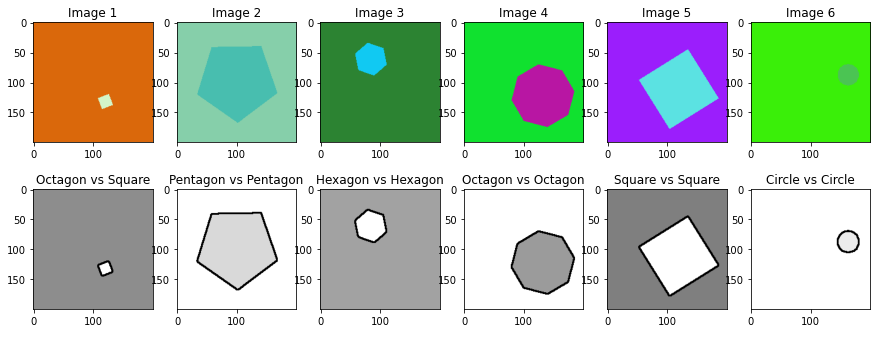
\includegraphics[width=\textwidth]{Figures/BatchExemple}
		\caption{Batch de 6 images}
		\label{fig:batchexemple}
	\end{figure}
	
	En sortie du script un pourcentage de réussite est donnée (voir figure \ref{fig:moyennebatchs}) où la moyenne des figures correspond à la moyenne des batchs.
	
	\begin{figure}[h]
		\centering
		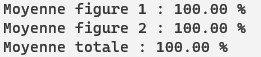
\includegraphics[width=0.5\linewidth]{Figures/MoyenneBatchs}
		\caption{Exemple de moyenne des batchs d'images}
		\label{fig:moyennebatchs}
	\end{figure}
	
	
	\paragraph{Description des paramètres : } Les paramètres principaux que j'ai fait varier sont les seuils d'hysteresis de la fonction canny d'openCV. Cette fonction est un filtrage qui capture les valeurs de bord qui fluctuent au-dessus et au-dessous des valeurs seuil \textbf{\textit{Tlow}} et \textbf{\textit{Thigh}}.
	
	\paragraph{Mesures : }
	\begin{center}
		\begin{tabular}{l l | l l}
			Réglage 1 & Réglage 2 & Mode Mesure & Moyenne de réussite \\
			\hline
			\textit{\textbf{Tlow}} = 10\quad\textit{\textbf{Thigh}} = 50 &  Convertis en B+W & 10img 10batchs & 51\%, 61.36\%, 70.75\% \\
			\textit{\textbf{Tlow}} = 10\quad\textit{\textbf{Thigh}} = 50 &  Convertis en B+W & 20img 20batchs & 62.42\% \\
			\textit{\textbf{Tlow}} = 10\quad\textit{\textbf{Thigh}} = 50 & Lis/charge en B+W & 20img 20batchs & 65.81\% \\
			\textit{\textbf{Tlow}} = 10\quad\textit{\textbf{Thigh}} = 30 & Lis/Charge en B+W & 20img 20batchs & 62.94\% \\
			\textit{\textbf{Tlow}} = 07\quad\textit{\textbf{Thigh}} = 45 & Lis/Charge en B+W & 20img 20batchs & 65\% \\
			\textit{\textbf{Tlow}} = 09\quad\textit{\textbf{Thigh}} = 45 & Lis/Charge en B+W & 20img 20batchs & 65.21\% \\
			\textit{\textbf{Tlow}} = 20\quad\textit{\textbf{Thigh}} = 40 & Lis/Charge en B+W & 20img 20batchs & 62.2\% \\
		\end{tabular}
	\end{center}
	
	Le réglage 2 est un test directement dans l'algorithme pour voir si il y avait une différence entre convertir l'image en 2 couleurs ou charger l'image en 2 couleurs, or il n'y a pas de différence visible dans les test.
	
	On peut voir que le taux de réussite n'est pas encore optimale mais ne descends presque jamais en dessous des 60\% sur une moyenne de 400 images ce qui me convient suffisamment pour continuer sur la suite du projet. J'ai décidé de conserver le mode \textit{\textbf{Tlow}} = 10 \textit{\textbf{Thigh}} = 50 avec \textit{Lis/charge en B+W} pour la version finale du script.

\subsection{Reconnaissance de formes - image réelles}

	\subsubsection{Images utilisées}
	
	\subsubsection{Explication du code}
	
	\subsubsection{Essais et étalonnage}
	
\subsection{Création de l'interface}

\clearpage	
\subsection{Description d'image - Machine learning}

\subsubsection{Model utilisé}

\subsubsection{Explication du code}

\clearpage	
\subsection{Application TKinter}

\subsubsection{Fonctionnement}

\subsubsection{Explication du code}

%---
\clearpage
\section{Conclusion}

